% **************************************************************************************************
% ** SPSC Report and Thesis Template
% **************************************************************************************************
%
% ***** Authors *****
% Daniel Arnitz, Paul Meissner, Stefan Petrik
% Signal Processing and Speech Communication Laboratory (SPSC)
% Graz University of Technology (TU Graz), Austria
%
% ***** Changelog *****
% 0.1   2010-01-25   extracted from report template by Daniel Arnitz (not ready yet)
% 0.2   2010-02-08   added thesis titlepage and modified layout (not ready yet)
% 0.3   2010-02-18   added TUG logo and statutory declaration
% 0.4   2010-02-18   moved the information fields below % **************************************************************************************************
% ** SPSC Report and Thesis Template
% **************************************************************************************************
%
% ***** Authors *****
% Daniel Arnitz, Paul Meissner, Stefan Petrik
% Signal Processing and Speech Communication Laboratory (SPSC)
% Graz University of Technology (TU Graz), Austria
%
% ***** Changelog *****
%
% ***** Todo *****
%
% **************************************************************************************************



\documentclass[%
a4paper,% !!! ATTENTION: geometry package below !!!
\Twosided,% !!! ATTENTION: geometry package below !!!
openany,% begin chapters with new right page (openright) or don't care (openany)
11pt,%
fleqn,% equations not centered, but on the left side
tablecaptionbelow,% captions below tables
% titlepage,% use title
pointlessnumbers,% do not generate point at the end of section numbers (e.g. 1.4.5 instead of 1.4.5.)
final,%
]{scrreprt}% (KOMA)

\usepackage[paper=a4paper,\Twosided,%
textheight=246mm,%
textwidth=160mm,%
heightrounded=true,% round textheight to multiple of lines (avoids overfull vboxes)
ignoreall=true,% do not include header, footer, and margins in calculations
marginparsep=5pt,% marginpar only used for signs (centered), thus only small sep. needed
marginparwidth=10mm,% prevent margin notes to be out of page
hmarginratio=2:1,% set margin ration (inner:outer for twoside) - (2:3 is default)
]{geometry}%


% master
\usepackage{ifthen}% for optional parts
\usepackage[utf8]{inputenc}% German special characters
\ifthenelse{\equal{\DocumentLanguage}{en}}{\usepackage[USenglish]{babel}}{}%
\ifthenelse{\equal{\DocumentLanguage}{de}}{\usepackage[ngerman]{babel}}{}%
\usepackage[%
headtopline,plainheadtopline,% activate all lines (header and footer)
headsepline,plainheadsepline,%
footsepline,plainfootsepline,%
footbotline,plainfootbotline,%
automark% auto update \..mark
]{scrpage2}% (KOMA)
\usepackage{makeidx}% used to make an index directory
\usepackage[]{caption}% customize captions
\usepackage{multicol}%
\usepackage[stable,bottom,hang,splitrule,multiple,symbol*]{footmisc}% customize footnotes


% text
\usepackage{varioref}% improved references
\usepackage{color}% e.g., for color boxes
\usepackage{rotating}% to rotate objects
\usepackage{gensymb}% symbols (perthousand, Celsius, ...)
\usepackage[right]{eurosym}% euro symbol on the right side (51 EUR)
\usepackage[normalem]{ulem}% cross-out, strike-out, underlines (normalem: keep \emph italic)
%\usepackage[safe]{textcomp}% loading in safe mode to avoid problems (see LaTeX companion)
%\usepackage[geometry,misc]{ifsym}% technical symbols
\usepackage{remreset}%\@removefromreset commands (e.g., for continuous footnote numbering)
\usepackage[%
breaklinks=true,% allow line break in links
colorlinks=true,% if false: framed link
linkcolor=black,anchorcolor=black,citecolor=black,filecolor=black,%
menucolor=black,urlcolor=black]{hyperref}% hyperlinks for references


% math
\usepackage{amsmath,amssymb,amstext,bm} % use math packages
\usepackage{mathcomp}% symbols (perthousand, ...) in math mode


% graphics
\usepackage{graphicx}% use simple graphics
\usepackage{subfigure}% subfigures (a),(b),(c)... within figures
\usepackage{flafter}% place floats always after reference
\usepackage{placeins}% preventing floats from crossing a barrier
\usepackage{float}% to place floats !HERE!
\usepackage{psfrag}% replace text in eps figures


% tables
\usepackage{hhline}% hline doesn't work with colored columns, so using hhline
\usepackage{longtable}% for tables longer than one page
\usepackage{dcolumn}% for number alignment in tables
\usepackage{colortbl}% color in tables


% listings
%\usepackage{alltt}% verbatim environment with commands available
\usepackage{listings}% program code listings


% other
%\usepackage{layout}% graphical page layout (spacings)
\usepackage{xspace}% add space after macros if not followed by punctuation character
\makeindex% used for index creation

 (encoding...)
% 0.5   2010-03-02   added \ShortTitle to fix problems with long thesis titles
%                    added \ThesisType (makes the template suitable for MSc, BSc, PhD, ... Thesis)
%
% ***** Todo *****
% - Introduction/Usage
% **************************************************************************************************

% **************************************************************************************************
% basic setup
\newcommand{\DocumentType}{report} % "thesis" / "report"
\newcommand{\DocumentLanguage}{de} % "en" / "de"
\newcommand{\Twosided}{} % "twoside" / ""


% **************************************************************************************************
% template setup -- do not change these unless you know what you are doing!
% **************************************************************************************************
% ** SPSC Report and Thesis Template
% **************************************************************************************************
%
% ***** Authors *****
% Daniel Arnitz, Paul Meissner, Stefan Petrik
% Signal Processing and Speech Communication Laboratory (SPSC)
% Graz University of Technology (TU Graz), Austria
%
% ***** Changelog *****
%
% ***** Todo *****
%
% **************************************************************************************************



\documentclass[%
a4paper,% !!! ATTENTION: geometry package below !!!
\Twosided,% !!! ATTENTION: geometry package below !!!
openany,% begin chapters with new right page (openright) or don't care (openany)
11pt,%
fleqn,% equations not centered, but on the left side
tablecaptionbelow,% captions below tables
% titlepage,% use title
pointlessnumbers,% do not generate point at the end of section numbers (e.g. 1.4.5 instead of 1.4.5.)
final,%
]{scrreprt}% (KOMA)

\usepackage[paper=a4paper,\Twosided,%
textheight=246mm,%
textwidth=160mm,%
heightrounded=true,% round textheight to multiple of lines (avoids overfull vboxes)
ignoreall=true,% do not include header, footer, and margins in calculations
marginparsep=5pt,% marginpar only used for signs (centered), thus only small sep. needed
marginparwidth=10mm,% prevent margin notes to be out of page
hmarginratio=2:1,% set margin ration (inner:outer for twoside) - (2:3 is default)
]{geometry}%


% master
\usepackage{ifthen}% for optional parts
\usepackage[utf8]{inputenc}% German special characters
\ifthenelse{\equal{\DocumentLanguage}{en}}{\usepackage[USenglish]{babel}}{}%
\ifthenelse{\equal{\DocumentLanguage}{de}}{\usepackage[ngerman]{babel}}{}%
\usepackage[%
headtopline,plainheadtopline,% activate all lines (header and footer)
headsepline,plainheadsepline,%
footsepline,plainfootsepline,%
footbotline,plainfootbotline,%
automark% auto update \..mark
]{scrpage2}% (KOMA)
\usepackage{makeidx}% used to make an index directory
\usepackage[]{caption}% customize captions
\usepackage{multicol}%
\usepackage[stable,bottom,hang,splitrule,multiple,symbol*]{footmisc}% customize footnotes


% text
\usepackage{varioref}% improved references
\usepackage{color}% e.g., for color boxes
\usepackage{rotating}% to rotate objects
\usepackage{gensymb}% symbols (perthousand, Celsius, ...)
\usepackage[right]{eurosym}% euro symbol on the right side (51 EUR)
\usepackage[normalem]{ulem}% cross-out, strike-out, underlines (normalem: keep \emph italic)
%\usepackage[safe]{textcomp}% loading in safe mode to avoid problems (see LaTeX companion)
%\usepackage[geometry,misc]{ifsym}% technical symbols
\usepackage{remreset}%\@removefromreset commands (e.g., for continuous footnote numbering)
\usepackage[%
breaklinks=true,% allow line break in links
colorlinks=true,% if false: framed link
linkcolor=black,anchorcolor=black,citecolor=black,filecolor=black,%
menucolor=black,urlcolor=black]{hyperref}% hyperlinks for references


% math
\usepackage{amsmath,amssymb,amstext,bm} % use math packages
\usepackage{mathcomp}% symbols (perthousand, ...) in math mode


% graphics
\usepackage{graphicx}% use simple graphics
\usepackage{subfigure}% subfigures (a),(b),(c)... within figures
\usepackage{flafter}% place floats always after reference
\usepackage{placeins}% preventing floats from crossing a barrier
\usepackage{float}% to place floats !HERE!
\usepackage{psfrag}% replace text in eps figures


% tables
\usepackage{hhline}% hline doesn't work with colored columns, so using hhline
\usepackage{longtable}% for tables longer than one page
\usepackage{dcolumn}% for number alignment in tables
\usepackage{colortbl}% color in tables


% listings
%\usepackage{alltt}% verbatim environment with commands available
\usepackage{listings}% program code listings


% other
%\usepackage{layout}% graphical page layout (spacings)
\usepackage{xspace}% add space after macros if not followed by punctuation character
\makeindex% used for index creation


\input{./base/layout_\DocumentType}
% **************************************************************************************************
% ** SPSC Report and Thesis Template
% **************************************************************************************************
%
% ***** Authors *****
% Daniel Arnitz, Paul Meissner, Stefan Petrik
% Signal Processing and Speech Communication Laboratory (SPSC)
% Graz University of Technology (TU Graz), Austria
%
% ***** Changelog *****
%
% ***** Todo *****
%
% **************************************************************************************************



% **************************************************************************************************
% * SECTIONING AND TEXT
% **************************************************************************************************

% new chapter, section, ... plus a few addons
%   part
\newcommand{\newpart}[2]{\FloatBarrier\cleardoublepage\part{#1}\label{part:#2}}%
%   chapter
\newcommand{\newchapter}[2]{\FloatBarrier\chapter{#1}\label{chp:#2}}
\newcommand{\newchapterNoTOC}[2]{\FloatBarrier\stepcounter{chapter}\chapter*{#1}\label{chp:#2}}%
%   section
\newcommand{\newsection}[2]{\FloatBarrier\vspace{5mm}\section{#1}\label{sec:#2}}%
\newcommand{\newsectionNoTOC}[2]{\FloatBarrier\vspace{5mm}\stepcounter{section}\section*{#1}\label{sec:#2}}%
%   subsection
\newcommand{\newsubsection}[2]{\FloatBarrier\vspace{3mm}\subsection{#1}\label{sec:#2}}%
\newcommand{\newsubsectionNoTOC}[2]{\FloatBarrier\vspace{3mm}\stepcounter{subsection}\subsection*{#1}\label{sec:#2}}%
%   subsubsection
\newcommand{\newsubsubsection}[2]{\vspace{2mm}\subsubsection{#1}\label{sec:#2}}%
\newcommand{\newsubsubsectionNoTOC}[2]{\vspace{2mm}\stepcounter{subsubsection}\subsubsection*{#1}\label{sec:#2}}%

% next paragraph
\newcommand{\nxtpar}{\par\bigskip}

% "stylish" quotes on the right side
\newcommand{\openingquote}[2]{\hfill\parbox[t]{10cm}{\itshape\raggedleft{"#1"}\\\footnotesize -- #2}\nxtpar}%

% direct quotes
% \newenvironment{directquote}{\nxtpar\hrule}{\hrule}\hfill\litref{#1}{#2}}

% warnings and attention signs in marginpar
\newcommand{\MDanger}{\marginpar{\Huge\centering\fbox{\textbf{!}}}}%
\newcommand{\MAttention}{\marginpar{\Huge\centering\textbf{!}}}%
\newcommand{\MHint}{\marginpar{\Huge\centering\textbf{\checkmark}}}%
\newcommand{\MQuestion}{\marginpar{\Huge\centering\textbf{?}}}%

% same footnote number as last one
\newcommand{\lastfootnotemark}{\addtocounter{footnote}{-1}\footnotemark}%

% value-unit commands (for 457 kHz, etc)
\newcommand{\vu}[2]{\mbox{$#1\,\text{#2}$}} % "value~unit" ... prevents e.g. 456 \linebreak mV
\newcommand{\vuc}[3]{\mbox{$#1\,\text{#2}\;#3\,\%$}} % "value~unit~tolerance-per-cent"
\newcommand{\vum}[3]{\mbox{$#1\,\text{#2}\;#3\,\perthousand$}} % "value~unit~tolerance-per-mil"

% reminders
\newcommand{\reminder}[1]{\colorbox{red}{#1}\xspace}%
\newcommand{\rem}{\reminder{(...)}}%
\newcommand{\remq}{\reminder{???}}%
\newcommand{\uc}{\nxtpar\colorbox{yellow}{... under construction ...}\nxtpar}%

% misc
\newcommand{\pwd}{.} % present working directory (can be used to create relativ paths per part, etc.)


% **************************************************************************************************
% * MATH
% **************************************************************************************************

% highlighting
\newcommand{\vm}[1]{\bm{#1}}% vector or matrix

% operators
\newcommand{\E}[1]{\text{E}\!\left\{#1\right\}}% expectation operator
\newcommand{\var}[1]{\text{var}\!\left\{#1\right\}}% variance operator
\renewcommand{\ln}[1]{\text{ln}\!\left(#1\right)}% natural logarithm
\newcommand{\ld}[1]{\text{ld}\!\left(#1\right)}% logarithm base 2
\renewcommand{\log}[1]{\text{log}\!\left(#1\right)}% logarithm (base 10)
\newcommand{\logb}[2]{\text{log}_{#1}\!\left(#2\right)}% logarithm base ...
\newcommand{\avgvar}[1]{\overline{\text{var}}\!\left\{#1\right\}}% average variance operator
\renewcommand{\Re}[1]{\text{Re}\!\left\{#1\right\}}% real part
\renewcommand{\Im}[1]{\text{Im}\!\left\{#1\right\}}% imaginary part

% other
\newcommand{\conj}{^\ast}% conjugate complex
\newcommand{\mtx}[2]{\left[\begin{array}{#1}#2\end{array}\right]}%vector/matrix


% **************************************************************************************************
% * FLOATS (FIGURES, TABLES, LISTINGS, ...)
% **************************************************************************************************

% figures without frames
%   standard
\newcommand{\fig}[3]{\begin{figure}\centering\includegraphics[width=\textwidth]{#1}\caption{#2}\label{fig:#3}\end{figure}}%
%   with controllable parameters
\newcommand{\figc}[4]{\begin{figure}\centering\includegraphics[#1]{#2}\caption{#3}\label{fig:#4}\end{figure}}%
%   two subfigures
\newcommand{\twofig}[6]{\begin{figure}\centering%
\subfigure[#2]{\includegraphics[width=0.495\textwidth]{#1}}%
\subfigure[#4]{\includegraphics[width=0.495\textwidth]{#3}}%
\caption{#5}\label{fig:#6}\end{figure}}%
%   two subfigures and controllable parameters
\newcommand{\twofigc}[8]{\begin{figure}\centering%
\subfigure[#3]{\includegraphics[#1]{#2}}%
\subfigure[#6]{\includegraphics[#4]{#5}}%
\caption{#7}\label{fig:#8}\end{figure}}%

% framed figures
%   standard
\newcommand{\figf}[3]{\begin{figure}\centering\fbox{\includegraphics[width=\textwidth]{#1}}\caption{#2}\label{fig:#3}\end{figure}}%
%   with controllable parameters
\newcommand{\figcf}[4]{\begin{figure}\centering\fbox{\includegraphics[#1]{#2}}\caption{#3}\label{fig:#4}\end{figure}}%
%   two subfigures
\newcommand{\twofigf}[6]{\begin{figure}\centering%
\fbox{\subfigure[#2]{\includegraphics[width=0.495\textwidth]{#1}}}%
\fbox{\subfigure[#4]{\includegraphics[width=0.495\textwidth]{#3}}}%
\caption{#5}\label{fig:#6}\end{figure}}%
%   two subfigures and controllable parameters
\newcommand{\twofigcf}[8]{\begin{figure}\centering%
\fbox{\subfigure[#3]{\includegraphics[#1]{#2}}}%
\fbox{\subfigure[#6]{\includegraphics[#4]{#5}}}%
\caption{#7}\label{fig:#8}\end{figure}}%

% listings
\newcommand{\filelisting}[4]{\lstinputlisting[print=true,language=#1,caption={#3},label={lst:#4}]{#2}}

% preserve backslash for linebreaks in tables (ragged... redefines \\, thus it has to be preserved)
\newcommand{\pbs}[1]{\let\temp=\\#1\let\\=\temp}%

\graphicspath{{./drawings/}{./plots/}{./images/}}
% **************************************************************************************************
% ATTENTION: Make sure that makeindex is set to -s "./base/index.sty"
% **************************************************************************************************

% uncomment to get watermarks:
% \usepackage[first,bottom,light,draft]{draftcopy}
% \draftcopyName{ENTWURF}{160}


% **************************************************************************************************
% information fields

% general
\newcommand{\DocumentTitle}{Computational Intelligence UE}
\newcommand{\DocumentSubtitle}{Homework 1: Linear Regression}
\newcommand{\ShortTitle}{CI Homework 1} % used in headers (keep short!)
\newcommand{\DocumentAuthor}{Thomas Ebner, Raphael Hoheneder, Stefan N\"ohmer}
\newcommand{\DocumentDate}{Graz, \today}
%    for thesis only (will be ignored for reports)
\newcommand{\ThesisType}{Master's Thesis}
\newcommand{\Organizations}{Signal Processing and Speech Communications Laboratory \\ Graz University of Technology \\[1cm] on behalf of \\ Some Company} % SPSC \\ TUG \\[1cm] on behalf of \\ A Nice Company
\newcommand{\Advisors}{Dipl.-Ing. Dr. Assoc.Prof. Klaus Witrisal \\ Dipl.-Ing. Paul Meissner} % Advisor 1 \\ Advisor 2 \\ ...
\newcommand{\Supervisors}{Univ.-Prof. Dipl.-Ing. Dr.techn. Gernot Kubin}

% revision number
\newcommand{\RevPrefix}{alpha~}
\newcommand{\RevLarge}{1}
\newcommand{\RevSmall}{1}

% confidential?
\newcommand{\ConfidNote}{confidential}% {"confidential", "eyes only", ...}

% short command for vectors
\newcommand{\vect}[1]{\mathbf{#1}}


\begin{document}

%listingstyle:
\definecolor{orange}{rgb}{0.75,0.65,0}
\definecolor{gruen}{rgb}{0,0.5,0}
\definecolor{listinggray}{gray}{0.97}
\definecolor{listingshadow}{gray}{0.2}
\lstloadlanguages{Matlab}
\lstset{frame=shadowbox,
		rulesepcolor=\color{listingshadow},
		numbers=left,
		basicstyle=\scriptsize\ttfamily,
		numberstyle=\tiny,
		keywordstyle=\color{blue}\bfseries, % bold black keywords
		identifierstyle=, % nothing happens
		commentstyle=\color{gruen}, % comments
		stringstyle=\color{orange}, % typewriter type for strings
		showstringspaces=false,
		tabsize=4,
		backgroundcolor=\color{listinggray}
        }

% **************************************************************************************************
% titlepage
\input{./base/titlepage_\DocumentType}

% statutory declaration for theses
\ifthenelse{\equal{\DocumentType}{thesis}}{% **************************************************************************************************
% ** SPSC Report and Thesis Template
% **************************************************************************************************
%
% ***** Authors *****
% Daniel Arnitz, Paul Meissner, Andreas Laesser, Stefan Petrik
% Signal Processing and Speech Communication Laboratory (SPSC)
% Graz University of Technology (TU Graz), Austria
%
% ***** Changelog *****
% 0.1   2010-02-18   created
% 0.2   2010-03-02   added German declaration
%
% ***** Todo *****
% **************************************************************************************************

\cleardoublepage
\pagestyle{empty}\pagenumbering{roman}

\vspace*{1cm}

% English
\ifthenelse{\equal{\DocumentLanguage}{en}}{
\begin{center}\Large\bfseries Statutory Declaration\end{center}\vspace*{1cm}
\noindent I declare that I have authored this thesis independently, that I have not used other than the declared sources$/$resources, and that I have explicitly marked all material which has been quoted either literally or by content from the used sources.
\par\vspace*{4cm}
\centerline{
\begin{tabular}{m{1.5cm}cm{1.5cm}m{3cm}m{1.5cm}cm{1.5cm}}
\cline{1-3} \cline{5-7}
 & date & & & & (signature) &\\
\end{tabular}}
}

% German
\ifthenelse{\equal{\DocumentLanguage}{de}}{
\begin{center}\Large\bfseries Eidesstattliche Erkl�rung\end{center}\vspace*{1cm}
Ich erkl�re an Eides statt, dass ich die vorliegende Arbeit selbstst�ndig verfasst, andere als die angegebenen Quellen$/$Hilfsmittel nicht benutzt, und die den benutzten Quellen w�rtlich und inhaltlich entnommene Stellen als solche kenntlich gemacht habe.
\par\vspace*{4cm}
\centerline{
\begin{tabular}{m{1.5cm}cm{1.5cm}m{3cm}m{1.5cm}cm{1.5cm}}
\cline{1-3} \cline{5-7}
 & Graz, am & & & & (Unterschrift) &\\
\end{tabular}}
}

}{}


% **************************************************************************************************
% **************************************************************************************************
% user-defined part

\chapter{Homework: Linear Regression}
\section{Linear Regression with Non-Linear Basis-Functions}
\subsection{Task 1.1.1: Polynomial Basis Functions}

\subsubsection{Aufgabenstellung:}


Es sollen die Gewichtungsfaktoren für Polynome vom 0ten Grad bis zum 18ten Grad gefunden werden, dazu sind die 60 gegebenen X- und Y-Trainingswerte zu verwenden.


Danach sind die Trainingspunkte, die Target-Funktion(y\_target) und die ``Lern-funktionen'' zu Auszugeben.


Die Basisfunktionen als Funktion von X ausgeben.

Ausgeben des ``Mean Squared Error'' (MSE) für die Trainings- und Test- werte.


\subsubsection{Plots \& Diskussion:}
\begin{figure}[hp!]
\begin{center}
 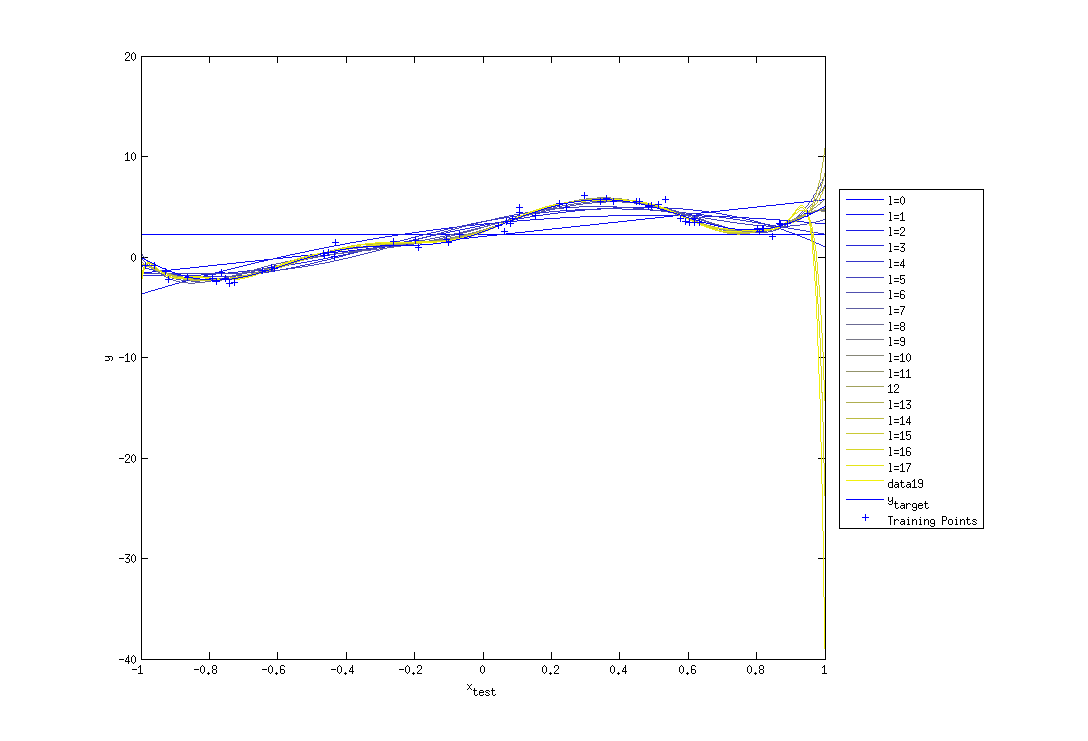
\includegraphics[width=0.99\textwidth]{./figures/1_1_1_unscaled_learn_fct}
 \caption[Unskalierte Lernfunktionen]{Unskalierte Lernfunktionen}
\label{fig:unscaled_learn_fct}
\end{center}
\end{figure}


\begin{figure}[hp!]
\begin{center}
 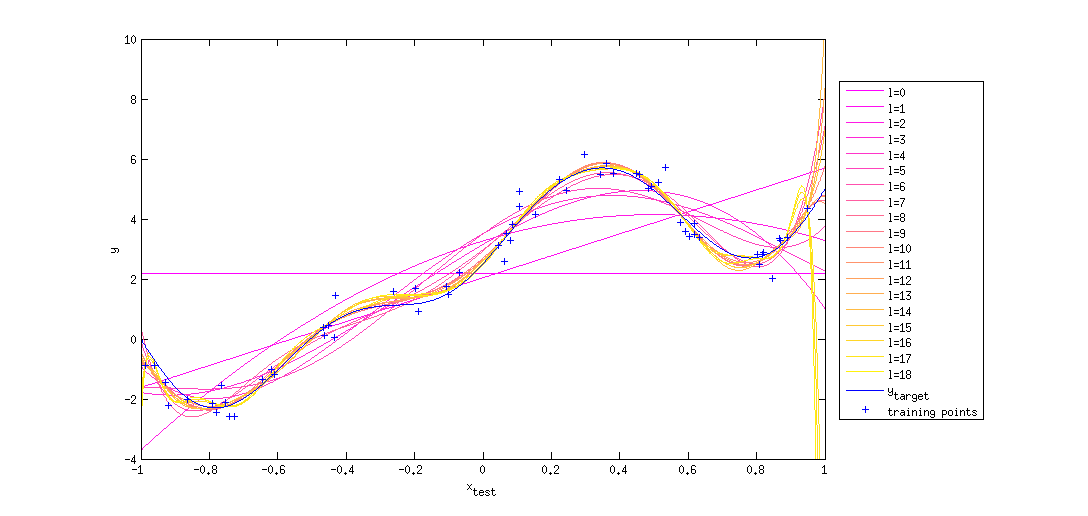
\includegraphics[width=1\textwidth]{./figures/1_1_1_scal_learn_fct}
 \caption[Skalierte Lernfunktionen]{Skalierte Lernfunktionen}
\label{fig:scal_learn_fct}
\end{center}
\end{figure}

In Abbildung \ref{fig:unscaled_learn_fct} sehen wir die Lernfunktionen.
In Abb. \ref{fig:unscaled_learn_fct} reisen die Werte für Polynome höheren Grades am Ende des ``Plots'' sehr stark aus.
 Das Bild wird somit in Y-Richtung gequetscht wird, in Abb. \ref{fig:scal_learn_fct} das ganze noch einmal skaliert um mehr zu erkennen.

\begin{figure}[hp!]
\begin{center}
 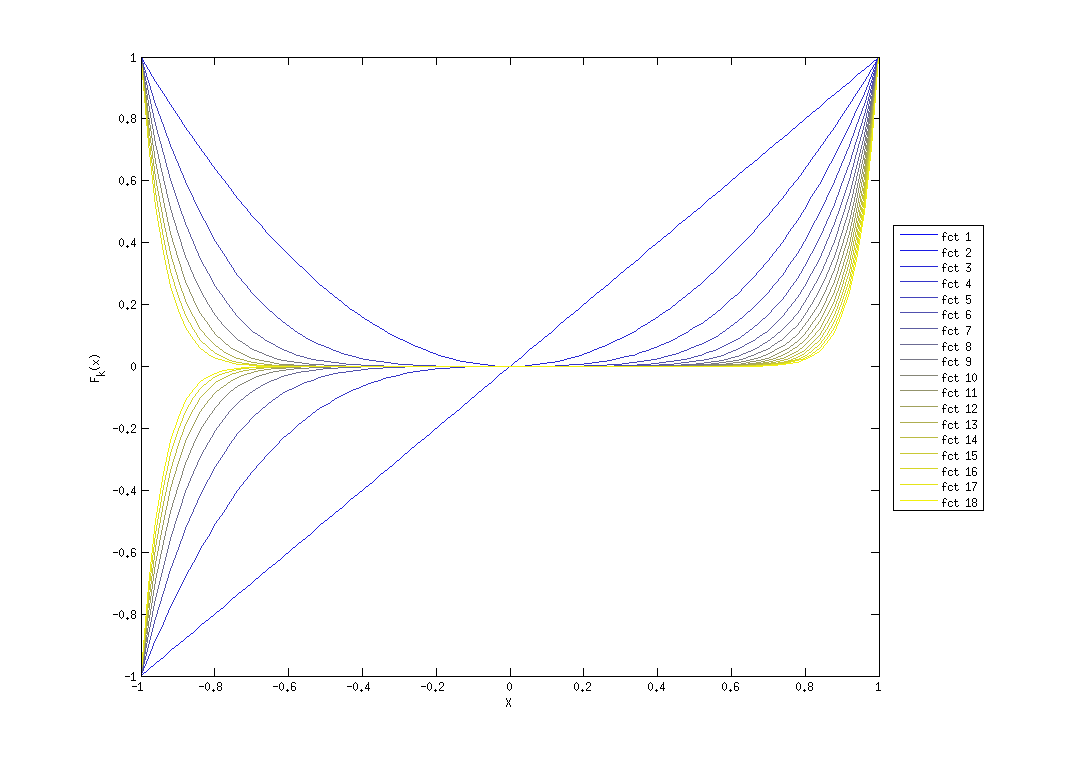
\includegraphics[width=1\textwidth]{./figures/1_1_1_base_fct}
 \caption[Basisfunktionen als Funktion von X]{Basisfunktionen als Funktion von X}
\label{fig:base_fct}
\end{center}
\end{figure}
In Abb. \ref{fig:base_fct} kann man Sehen das Funktionen höherer Ordnung sehr stark einknicken. Das bedeutet das sich Funktionen höherer Ordnung 
schneller bzw. stärker den Testdaten anpassen. Allerdings sollt hier ein Mittel gefunden werden, da die Testdaten ja auch nicht exakt und mit
Rauschen behaftet sind! 



Bei Funktionen mit höheren Polynomen ist die Funktion zwar sehr gut eingepasst an die Trainingspunkte, neigt aber zu starkem Überschwingen.
Das sog. ``Overfitting'' tritt hier auf.
\clearpage

\begin{figure}[hp!]
\begin{center}
 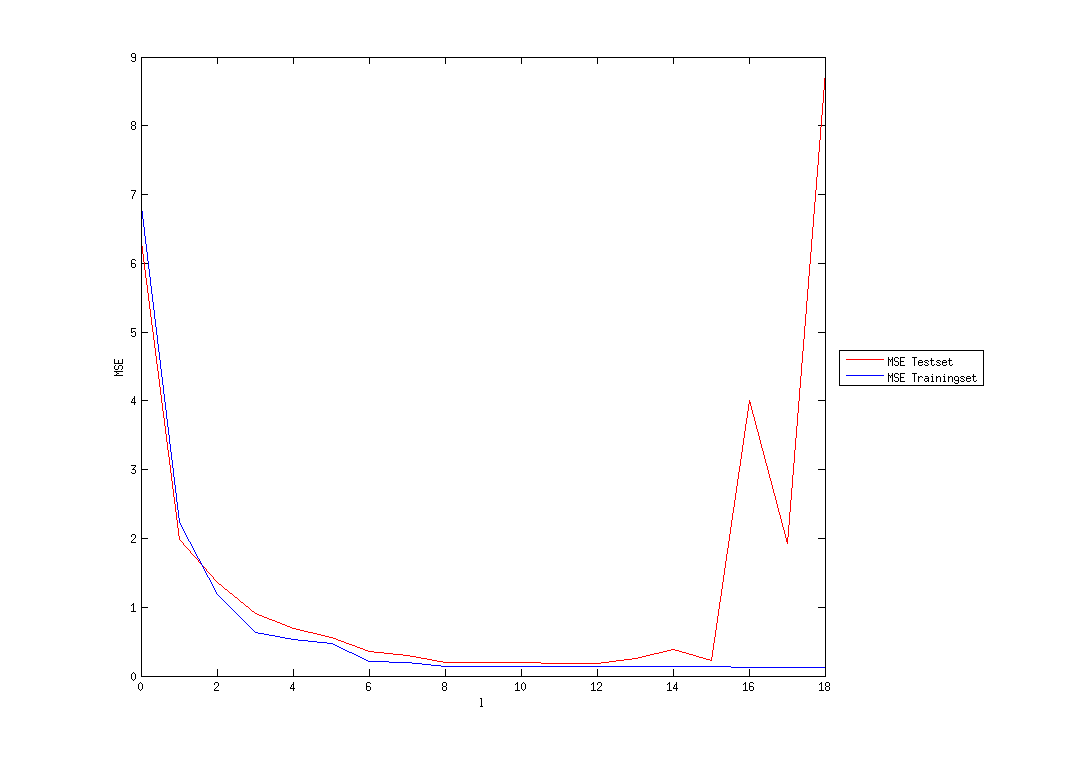
\includegraphics[width=1\textwidth]{./figures/1_1_1_MSE}
 \caption[Mean Square Error]{Mean Square Error für Trainings- und Test-Werte}
\label{fig:MSE}
\end{center}
\end{figure}

Wie man in Abb. \ref{fig:MSE} sehen kann ist bereits bei einer Funktion mit Grad 8 der Fehler sehr gering,bei Grad 8 ist  
Aufwand und Leistung am Besten. Es ist die Funktion nur für die Trainings-Werte 
perfekt angepasst allerdings wird durch das ``OverFitting'' für alle anderen Werte der Fehler wieder größer.
\subsection{Task 1.1.2: Radial Basis Functions}


\subsubsection{Aufgabenstellung:}
Nun ist die Basisfunktion ist nun eine Gau\ss{} 'sche Glockenkurve die mit $\phi_k(x) = exp(-(x-\mu_k)^2 /\sigma^2 )$ gegeben ist.
Wobei $d=2:18$, $\sigma$ $= 2/d$ und $\mu =d$ schritten zwischen -1 und 1 entspricht.
Es sind wieder  die Trainingspunkte, die Target-Funktion(y\_target) und die ``Lernfunktionen'' zu Auszugeben.
Die Basisfunktion mit $d=6,12$ und $18$ als Funktion von x Ploten.
Ausgeben des ``Mean Squared Error'' (MSE) für die Trainings- und Test- werte.



\subsubsection{Plots \& Diskussion:}


\begin{figure}[hp!]
\begin{center}
 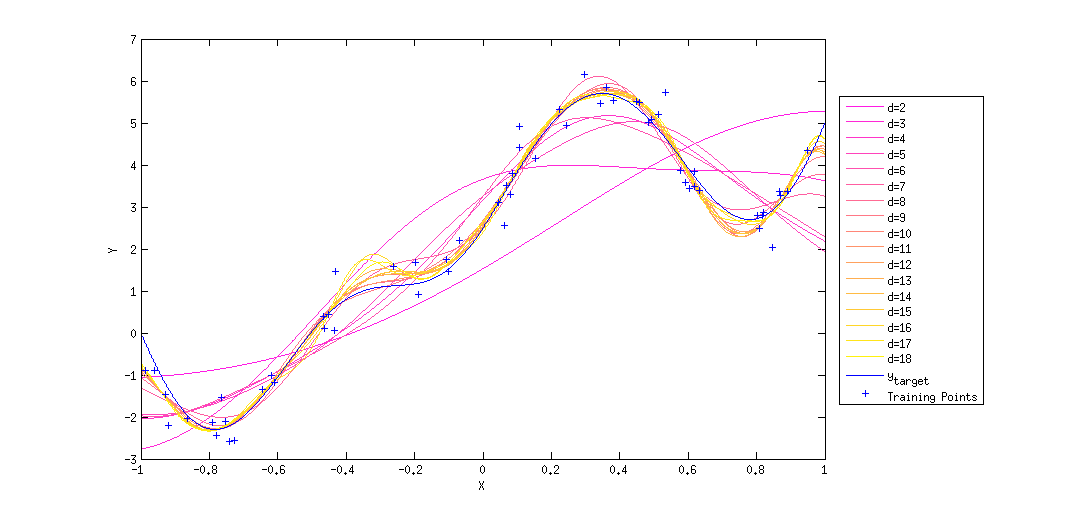
\includegraphics[width=1\textwidth]{./figures/RBF_learn}
 \caption[Trainingspunkte, Target-Funktion und Lernfunktionen]{Trainingspunkte, Target-Funktion und Lernfunktionen}
\label{fig:RBF_learn}
\end{center}
\end{figure}
Wie man in Abb. \ref{fig:RBF_learn} sehen kann ist das ``Ausbrechen'' bei der Radial-Funktion, am Ende, bei weitem nicht so ausgeprägt!

\clearpage
\begin{figure}[hp!]
\begin{center}
 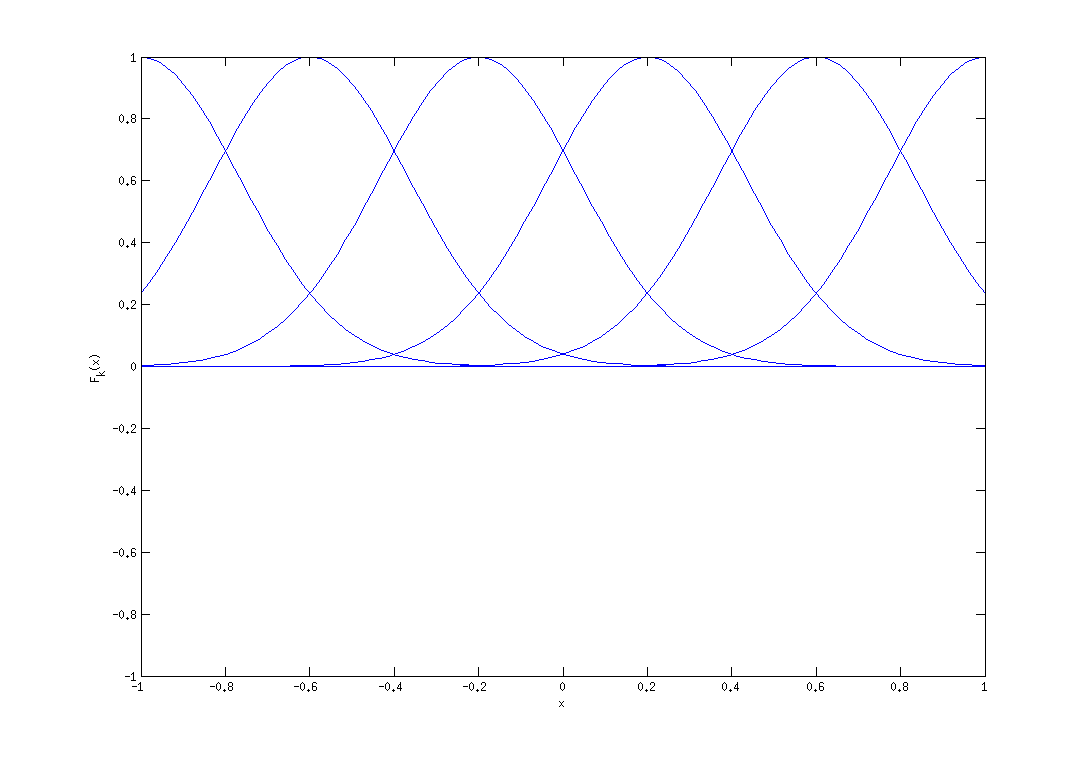
\includegraphics[width=10cm]{./figures/RBF_6}
 \caption[Basisfunktionen als Funktion von X (d=6)]{Basisfunktionen als Funktion von X mit einem $d=6$}
\label{fig:RBF_6}
\end{center}
\end{figure}

\begin{figure}[hp!]
\begin{center}
 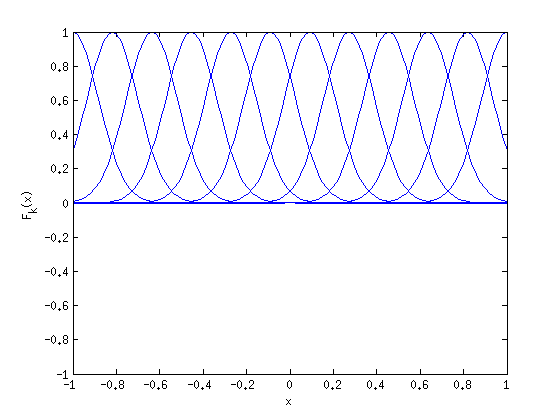
\includegraphics[width=10cm]{./figures/RBF_12}
 \caption[Basisfunktionen als Funktion von X, d=12]{Basisfunktionen als Funktion von X mit einem $d=12$}
\label{fig:RBF_12}
\end{center}
\end{figure}


\begin{figure}[hp!]
\begin{center}
 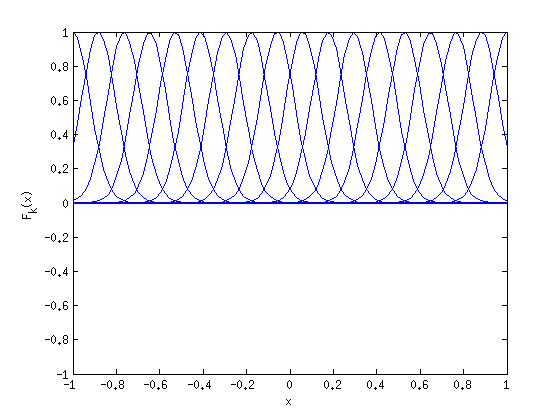
\includegraphics[width=10cm]{./figures/RBF_18}
 \caption[Basisfunktionen als Funktion von X, d=18]{Basisfunktionen als Funktion von X mit einem $d=18$}
\label{fig:RBF_18}
\end{center}
\end{figure}
Man kann erkennen das auch hier bei höherer Ordnung die Steilheit zunimmt. Gau\ss{}'sche-funktionen neigen allerdings nicht zum ``ausbrechen''
da sie wenn sie Richtung unendlich gehen keinen ``Schaden'' anrichten, da sie wieder zu ihrem Nullpunkt zurückkehren.


\begin{figure}[hp!]
\begin{center}
 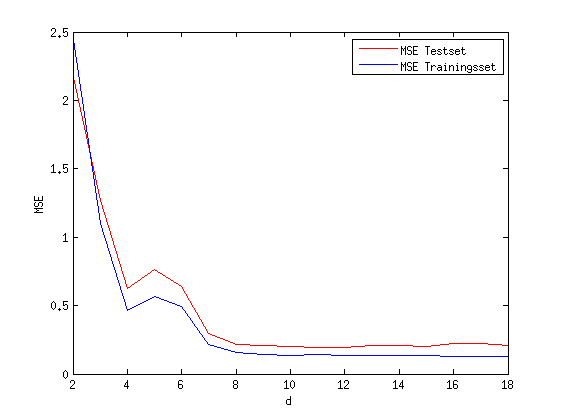
\includegraphics[width=0.7\textwidth]{./figures/RBF_MSE}
 \caption[MSE]{MSE des Trainingsset und des Testsets.}
\label{fig:RBF_MSE}
\end{center}
\end{figure}
\clearpage
\subsection{Task 1.1.3: Local Linear Models}

In diesem Beispiel ist die Designmatrix X doppelt so groß wie vorher. War sie in Task 1.1.2 noch $(60 \times d)$ groß, ist sie jetzt $(60 \times 2d)$. Neben den unskalierten Gausskurven gibt es nun auch ein zweites Set von Basisfunktionen: die Gausskurven von vorher, linear skaliert mit $x$.

Die Implementierung in Matlab ist der von Task 1.1.2 sehr ähnlich, es wurde nur eine zweite Designmatrix generiert, die der normalen Designmatrix entspricht, aber mit $x$ multipliziert wurde. Mit dem Klammer-Operator \texttt{[]} wurden die beiden Matrizen dann zu einer Matrix verbunden.

Abbildung~\ref{fig:113-curves-out} zeigt die Datenpunkte, die tatsächliche Funktion und die gelernte Funktion für unterschiedliche Anzahl von Basisfunktionen. Man erkennt, dass die Annäherung bei einer geringen Anzahl von Basisfunktionen nicht besonders gut ist, aber dann mit steigender Anzahl von Basisfunktionen sehr gut wird. Ist jedoch die Anzahl zu hoch, wird die Annäherung auch sehr schlecht.

Da Abbildung~\ref{fig:113-curves-out} auf alle Kurven skaliert wurde, erkennt man die angenäherte Funktion nicht besonders gut. Abbildung~\ref{fig:113-curves-in} zeigt die gleichen Kurven bei einer sinnvolleren Skalierung.

\begin{figure}[h!]
  \centering
  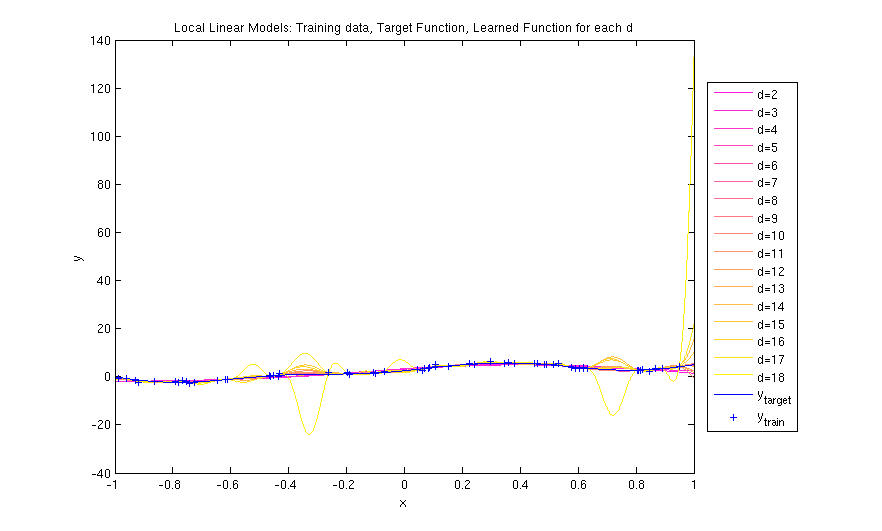
\includegraphics[width=\textwidth]{./figures/1_1_3_curves_out.png}
  \caption{Trainings-Punkte, Target-Funktion \& gelernte Funktion}
  \label{fig:113-curves-out}
\end{figure}

\begin{figure}[h!]
  \centering
  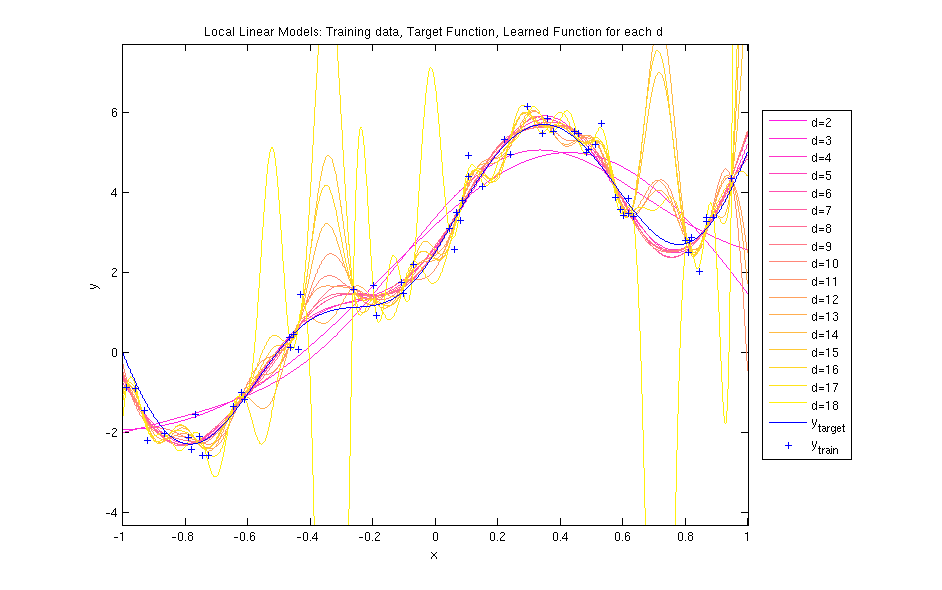
\includegraphics[width=\textwidth]{./figures/1_1_3_curves_in.png}
  \caption{Trainings-Punkte, Target-Funktion \& gelernte Funktion (skaliert)}
  \label{fig:113-curves-in}
\end{figure}

Diese Kurven sind aus einer gewissen Anzahl Basisfunktionen zusammengestellt, wobei die folgenden Abbildung diese Basisfunktionen visualisieren. Abbildung~\ref{fig:113-basis-6} zeigt die Verteilung von 6 Basisfunktionen, Abbildung~\ref{fig:113-basis-12} zeigt die Verteilung von 12 Basisfunktionen und Abbildung~\ref{fig:113-basis-18} zeigt die Verteilung von 18 Basisfunktionen.

\begin{figure}[h!]
  \centering
  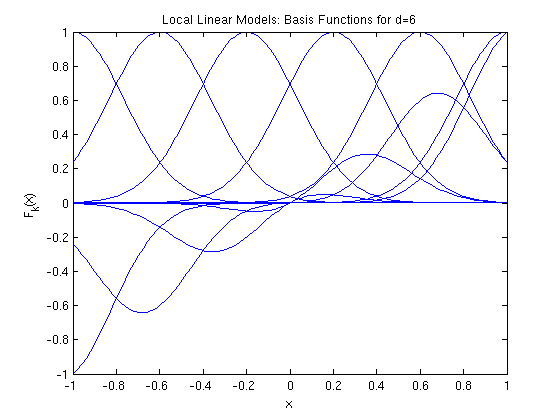
\includegraphics[width=0.5\textwidth]{./figures/1_1_3_basis_6.png}
  \caption{Aufteilung von 6 Basisfunktionen $\Phi_k(x)$}
  \label{fig:113-basis-6}
\end{figure}

\begin{figure}[h!]
  \centering
  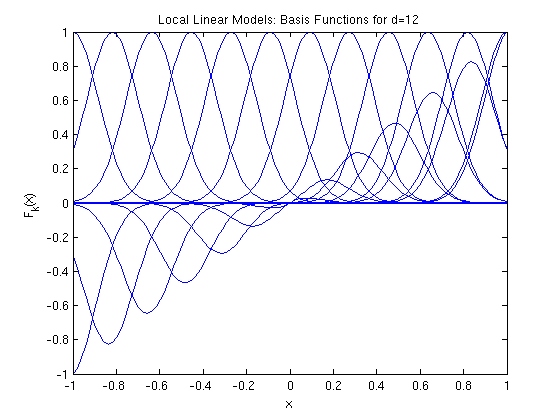
\includegraphics[width=0.5\textwidth]{./figures/1_1_3_basis_12.png}
  \caption{Aufteilung von 12 Basisfunktionen $\Phi_k(x)$}
  \label{fig:113-basis-12}
\end{figure}

\begin{figure}[h!]
  \centering
  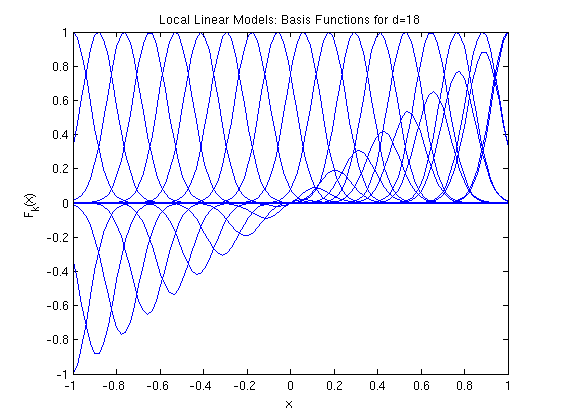
\includegraphics[width=0.5\textwidth]{./figures/1_1_3_basis_18.png}
  \caption{Aufteilung von 18 Basisfunktionen $\Phi_k(x)$}
  \label{fig:113-basis-18}
\end{figure}

Abbildung~\ref{fig:113-mse-out} zeigt den Mean Squared Error (MSE) bei den Trainings- und Testdaten in Abhängigkeit von der Anzahl der Basisfunktionen. Wie man auch in Abbildung~\ref{fig:113-curves-out} und Abbildung~\ref{fig:113-curves-in} erkennt, funktioniert die Annäherung für mittelgroße Werte von $l$ (Anzahl der Basisfunktionen) am besten. In Abbildung~\ref{fig:113-mse-out} erkennt man, wie extrem schlecht die Annäherung mit großen $l$ funktioniert. Passend skaliert ist der MSE in Abbildung~\ref{fig:113-mse-in} dargestellt. Ein sehr niedriger MSE ist bei $l=4$ Basisfunktionen erreichbar, wodurch durch den niedrigen Grad auch nur ein geringer Aufwand entsteht.

\begin{figure}[h!]
  \centering
  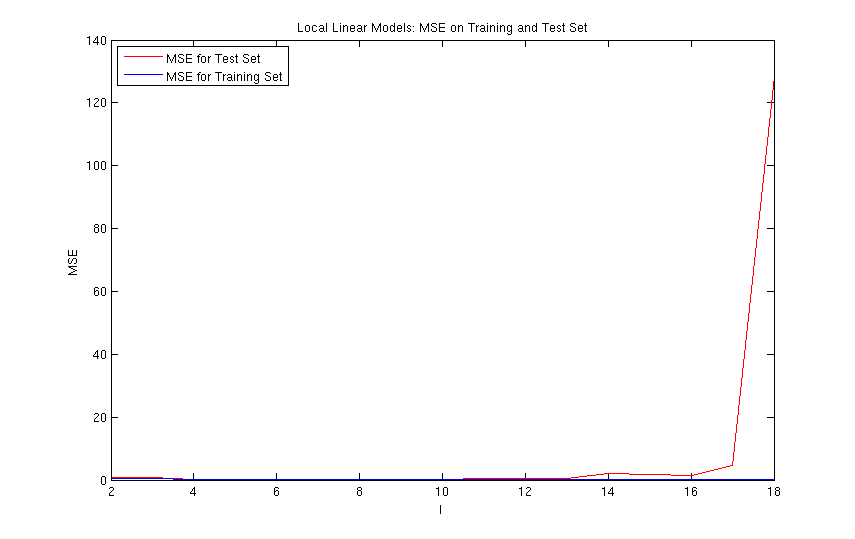
\includegraphics[width=\textwidth]{./figures/1_1_3_mse_out.png}
  \caption{MSE in Abhängigkeit von $l$}
  \label{fig:113-mse-out}
\end{figure}

\begin{figure}[h!]
  \centering
  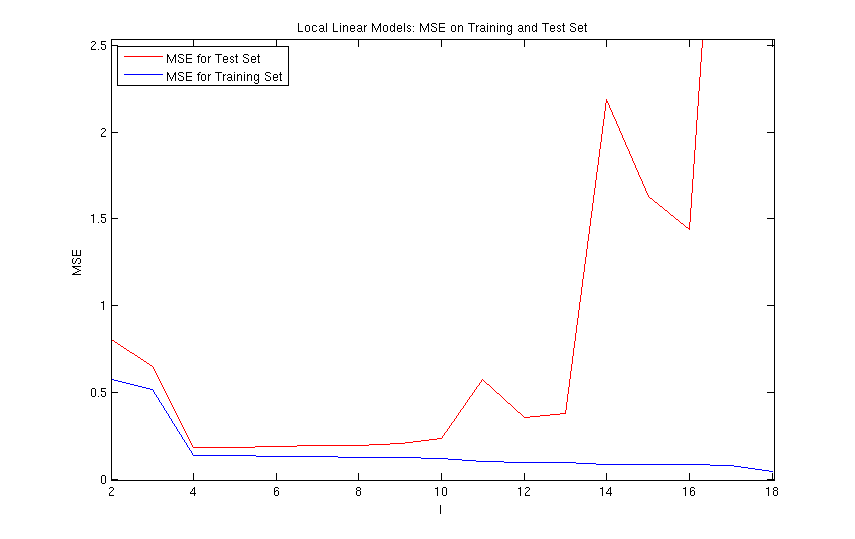
\includegraphics[width=\textwidth]{./figures/1_1_3_mse_in.png}
  \caption{MSE in Abhängigkeit von $l$ (skaliert)}
  \label{fig:113-mse-in}
\end{figure}

\clearpage

\paragraph{Vergleich zwischen den verschiedenen Basisfunktionen}

Den kleinsten MSE lieferten die Basisfunktionen in Task 1.1.2 und 1.1.3, wobei bei Task 1.1.2 die Gesamtperformance
über alle Ordnungen betrachtet sehr gut war. Bei Task 1.1.1 wird ein ähnlich gutes Ergebnis erst ab höherer Ordnung
erzielt. Die Basisfunktionen aus Task 1.1.3 ist für niedrigen Ordnungen bis ca. 12 gut, aber wird danach ziehmlich
schnell unbrauchbar. Für höhere Ordnung empfiehlt es sich den in Task 1.1.4 beschriebenen Faktor $\alpha$ einzuführen.

\subsection{Task 1.1.4: Regularized Polynomial Regression}

%nöhmes stuff:

\paragraph{Regularized Regression Grundlagen}

Folgende Fehlerfunktion soll minimal werden:

$$ E(\vect{w}) = \frac{1}{N} \sum_{i=1}^N(y_i - \sum_{k=1}^d \Phi_k(x_i) w_k)^2 + \alpha^2 \sum_{k=1}^d w_k^2 $$

Zuerst müssen die indizierten Variablen in Vektoren umgeschrieben werden:

$$ \vect{x} = \begin{bmatrix} x_1 \\ x_2 \\ \vdots \\ x_N \end{bmatrix}, \; \vect{y} = \begin{bmatrix} y_1 \\ y_2 \\ \vdots \\ y_N \end{bmatrix}, \; \vect{w} = \begin{bmatrix} w_1 \\ w_2 \\ \vdots \\ w_d \end{bmatrix}, \; \vect{\Phi}(\vect{x}) = \begin{bmatrix} \Phi_1(\vect{x}) \\ \Phi_2(\vect{x}) \\ \vdots \\ \Phi_d(\vect{x}) \end{bmatrix} $$

wobei $ \vect{x} \in M(N \times 1), \; \vect{y} \in M(N \times 1), \; \vect{w} \in M(d \times 1), \; \vect{\Phi}(\vect{x}) \in M(d \times 1) $.

Nun können die Summen in Matrixform umgeschrieben werden (von innen nach aussen):

$$ \sum_{k=1}^d \Phi_k w_k = \vect{\Phi}^T \cdot \vect{w}, \; \text{da} \begin{bmatrix} \Phi_1 && \Phi_2 && \hdots && \Phi_d \end{bmatrix} \cdot \begin{bmatrix} w_1 \\ w_2 \\ \vdots \\ w_d \end{bmatrix} = \Phi_1 w_1 + \Phi_2 w_2 + \hdots + \Phi_d w_d $$

$$ \alpha^2 \sum_{k=1}^d w_k^2 = \alpha^2 \cdot \vect{w}^T \cdot \vect{w}, \; \text{aus dem selben Grund wie oben} $$

Mit der gleichen Regel kann man auch die äußere Summe zusammenfassen:

$$ \sum_{i=1}^N (y_i - \sum_{k=1}^{d} \Phi_k(x_i) w_k)^2 = (\vect{y} - \vect{\Phi}(\vect{x})^T \vect{w})^T (\vect{y} - \vect{\Phi}(\vect{x})^T \vect{w}) $$

Also ergibt sich die gesamte Fehlerfunktion als:

$$ E(\vect{w}) = \frac{1}{N} (\vect{y} - \vect{\Phi}(\vect{x})^T \vect{w})^T (\vect{y} - \vect{\Phi}(\vect{x})^T \vect{w}) + \alpha^2 \vect{w}^T \vect{w} $$

Die Matrix $ \vect{\Phi}(\vect{x})^T $ wird im folgenden als Designmatrix $ \vect{X} $ abgekürzt und hat folgende Form:

$$ \vect{X} = \vect{\Phi}(\vect{x})^T = \begin{bmatrix} \Phi_1(x_1) && \Phi_2(x_1) && \hdots && \Phi_d(x_1) \\  \Phi_1(x_2) && \Phi_2(x_2) && \hdots && \Phi_d(x_2) \\ \vdots && \ddots \\ \Phi_1(x_N) && \Phi_2(x_N) && \hdots && \Phi_d(x_N) \end{bmatrix} $$

Ihre Dimension ist also $ \vect{X} \in M(N \times d) $.

Um nun den Fehler zu minimieren, muss die Fehlerfunktion abgeleitet werden:

$$ \frac{\partial E(\vect{w})}{\partial \vect{w}} = \frac{\partial}{\partial \vect{w}} \frac{1}{N} (\vect{y} - \vect{X} \vect{w})^T (\vect{y} - \vect{X} \vect{w}) + \alpha^2 \vect{w}^T \vect{w} $$

Mit $ \frac{\partial \vect{w}^T \vect{w}}{\partial \vect{w}} = 2 \vect{w}^T $ (Matrix-Cookbook, (10)) ergibt sich (innere Ableitung nicht vergessen!):

$$ \frac{\partial E(\vect{w})}{\partial \vect{w}} = - \frac{2}{N} (\vect{y} - \vect{X} \vect{w})^T \vect{X} + 2 \alpha^2 \vect{w}^T $$

Um das Minimum zu finden, wird diese Ableitung jetzt 0 gesetzt und auf $\vect{w}$ umgeformt:

$$ - \frac{2}{N} (\vect{y} - \vect{X} \vect{w})^T \vect{X} + 2 \alpha^2 \vect{w}^T = 0 $$
$$ \frac{2}{N} (\vect{y} - \vect{X} \vect{w})^T \vect{X} = 2 \alpha^2 \vect{w}^T $$
$$ (\vect{y} - \vect{X} \vect{w})^T \vect{X} = N \alpha^2 \vect{w}^T $$
$$ (\vect{y}^T - \vect{w}^T \vect{X}^T) \vect{X} = N \alpha^2 \vect{w}^T $$
$$ \vect{y}^T \vect{X} - \vect{w}^T \vect{X}^T \vect{X} = N \alpha^2 \vect{w}^T $$
$$ \vect{w}^T \vect{X}^T \vect{X} + N \alpha^2 \vect{w}^T = \vect{y}^T \vect{X} $$
$$ \vect{w}^T \vect{X}^T \vect{X} + \vect{w}^T N \alpha^2 = \vect{y}^T \vect{X} $$
$$ \vect{w}^T (\vect{X}^T \vect{X} + N \alpha^2 \vect{I}) = \vect{y}^T \vect{X} $$
$$ \vect{w}^T = \vect{y}^T \vect{X} (\vect{X}^T \vect{X} + N \alpha^2 \vect{I})^{-1} $$
$$ \vect{w} = (\vect{X}^T \vect{X} + N \alpha^2 \vect{I})^{-1} \vect{X}^T \vect{y} $$
%endlich!!! :)


%tom stuff:



\paragraph{Polynomial Basis Functions}




\clearpage
\newpage

\chapter{Listings}
\section{Polynomial basis functions}
\lstinputlisting[language=matlab]{../implementation/hw111.m}
\section{Radial basis functions}
\lstinputlisting[language=matlab]{../implementation/hw112.m}
\section{Local linear Models}
\lstinputlisting[language=matlab]{../implementation/hw113.m}
\section{Regularized Polynomial Regression}
\lstinputlisting[language=matlab]{../implementation/hw114.m}





% **************************************************************************************************
% **************************************************************************************************

%\appendix
%\bibliographystyle{/.base/ieeetran}
%\bibliography{_bibliography}

% place all floats and create label on last page
\FloatBarrier\label{end-of-document}
\end{document}

